SHArP \cite{sharp} stands for \textit{Scalable Hierarchical Aggregation Protocol}, and it defines a protocol for reduction operations.
This solutions aims to accelerate \gls{hpc} applications by offloading some operations to the network. SHArP \cite{sharp} is targeted to support the two most used \glspl{api} in the \gls{hpc} area today: MPI \cite{mpi} and OpenSHMEM \cite{openshmem}.
The kind of operations that can be offloaded to the network are:
\begin{mylist}
    \item MPI \cite{mpi} barrier, reduce and allreduce,
    \item logic operands like sum, min, max, or, xor, and,
    \item integer and floating-point operations
\end{mylist}.

\subsubsection{Details}
\paragraph{Entities}
\glspl{an} are logical entities performing reduction operations.
Such a node can either execute on a network device or on a server, and it is implemented as a daemon, namely \texttt{sharpd}.

\begin{figure}[!htb]
    \centering
        % trim = left, bottom, right, top
        \includegraphics[page=13, clip, trim=3.6cm 1.3cm 3.6cm 4.8cm, width=1.00\textwidth]{figures/analysis/inp/solutions.pdf}
    \caption{SHArP's \texorpdfstring{\cite{sharp}}{} basic topology and entities}
\end{figure}

All \glspl{an} must form an aggregation tree.
Multiple trees are allowed in a system.
Similarly to other in-network aggregation solutions like Daiet \cite{daiet}, data is aggregated along the aggregation tree by \glspl{an}, until it reaches a root \gls{an} that is in charge of distributing the result.

\begin{figure}[!htb]
    \centering
        % trim = left, bottom, right, top
        \includegraphics[page=15, clip, trim=3.3cm 0.9cm 1.6cm 4.6cm, width=1.00\textwidth]{figures/analysis/inp/solutions.pdf}
    \caption{SHArP's \texorpdfstring{\cite{sharp}}{} logical communication pattern}
\end{figure}

The protocol also introduces the concept of \textit{group}, consisting in a subset of physical hosts that are connected to the tree leaves: for instance, in MPI \cite{mpi} a group coincides with a \textit{communicator}.
One aggregation tree supports multiple groups.

Resources are managed by a special management entity called \gls{am}.
Faults and errors are always notified to this node, that will also take care of freeing all resources belonging to the tree in which the error occurred.
The detection of faults and errors cannot be done using timeouts since \gls{hpc} \glspl{api} do not bound the duration of aggregation operations: this is why faults must be necessarily detected by monitoring.

\paragraph{Data flow}
Eventually, an host program will need to execute a job on multiple nodes.
When the job is launched and all host processes have been created (e.g., a communicator in MPI \cite{mpi}), either the cluster resource manager (like Slurm \cite{slurm} or \glsdesc{ibm} Spectrum LSF) or an MPI \cite{mpi} launcher like \texttt{mpirun} will contact the \gls{am}, which will dedicate SHArP \cite{sharp} resources to the job and return back the list of these allocated resources.
At this point, a SHArP \cite{sharp} group has been created.
Each SHArP \cite{sharp} daemon \texttt{sharpd} running on every group member will establish a reliable connection to the dedicated leaf switch.
The \gls{am} informs the \glspl{an} about the switch resources allocated to the application, not allowing it to exceed the allocation.\par
Once connections have been established, all group members send an aggregation request message to their parent \gls{an}.
Each \gls{an} waits for all its children requests before sending the aggregated data piggybacked on another aggregation request to the parent node.
\glspl{an} temporarily maintain a data structure to track an aggregation operation's progress.\par
As soon as the tree root node receives data from all its children, it performs the final aggregation and it sends the result to a destination, that could be
\begin{mylist}
    \item one or more process belonging to one or more groups or
    \item an external process not belonging to any reduction group
\end{mylist}.
In the former case, the aggregation tree is used to redistribute the result.

\subsubsection{Implementation}
SHArP \cite{sharp} has been implemented using InfiniBand \cite{infiniband} as communication standard with \glsdesc{switchib2} devices, which provide support for data reduce operations and for barriers.
Nodes in the SHArP \cite{sharp} tree are InfiniBand \cite{infiniband} end nodes, and links are implemented using InfiniBand's \cite{infiniband} \textit{Reliable Connection}s.
When distributing a result using a multicast address, though, an unreliable delivery mechanism is used.
One \gls{an} can participate to at most 64 different aggregation trees.

\subsubsection{Minimum system requirements}
\glspl{an} (usually run by network devices) must form a tree whose leaves are connected to data producers (a \textit{communicator} in MPI \cite{mpi}).
Each data producer is connected to only one tree leaf.
The root \gls{an}, instead, is connected to the data consumer, which receives the final aggregated result.
\glspl{an} must dedicate part of their local memory to the system.

\begin{figure}[!htb]
    \centering
        % trim = left, bottom, right, top
        \includegraphics[page=14, clip, trim=2.4cm 0.7cm 1.8cm 3.6cm, width=1.00\textwidth]{figures/analysis/inp/solutions.pdf}
    \caption{SHArP's \texorpdfstring{\cite{sharp}}{} extended topology}
\end{figure}

The special management unit (\gls{am}) must act as a SHArP \cite{sharp} \gls{rm}, dedicating SHArP \cite{sharp} resources to those entities who request for them.

\begin{figure}[!htb]
    \centering
        % trim = left, bottom, right, top
        \includegraphics[page=16, clip, trim=3.6cm 0.3cm 3.7cm 0.2cm, width=1.00\textwidth]{figures/analysis/inp/solutions.pdf}
    \caption{Messages exchanged during a SHArP \texorpdfstring{\cite{sharp}}{} instance execution}
\end{figure}

\subsubsection{Conclusions}
For MPI \cite{mpi} applications SHArP \cite{sharp} brings a significant advantage in terms of latency: tests show that the latency improvement factor (latency experienced without SHArP \cite{sharp} divided by the one experienced with SHArP \cite{sharp}) is proportional to the message size.
Even in the worst case, with a message size of just \SI{8}{\mega\byte}, an MPI \cite{mpi} execution with SHArP \cite{sharp} is twice as fast as the one without using it.